


\documentclass[11pt]{article}
\usepackage[english]{babel}
\usepackage[utf8]{inputenc}
\usepackage{amssymb,amsmath}
\usepackage{fancyhdr}
\usepackage{a4wide}
\usepackage{epstopdf}
\usepackage[T1]{fontenc}
\usepackage{url} %% pour citer les url par \url
\usepackage{multirow} %% pour regrouper un texte sur plusieurs lignes dans une
\usepackage{color}
\usepackage{caption}
\usepackage{subfigure}
\usepackage{array}
\usepackage{import}
\usepackage[final]{pdfpages}
\usepackage{eso-pic}
\usepackage{xkeyval}
\usepackage{picture}
\usepackage{import}
\usepackage{subfigure}
\usepackage{titlesec}
\usepackage{multicol}
\usepackage{enumitem}
\usepackage{tikz,pgfplots,pgf}

\usetikzlibrary{arrows,shapes,arrows,positioning,calc,trees,snakes,plotmarks}

% nouveaux environements de theoreme
%----------------------
% nouvelles commandes
%----------------------
\newcommand{\promotion}{ truc}
\newcommand{\formationshort}{SARII}
\newcommand{\formationlong}{Systèmes Automatisés, Réseaux et Informatique Industrielle}
\newcommand{\departement}{GEII}

\newenvironment{objectif}{\noindent
\begin{lrbox}{\fmbox}\begin{minipage}{1.0\textwidth}\textbf{Objectifs}:}
{\end{minipage}\end{lrbox}\fbox{\usebox{\fmbox}}}



%\captionsfrenchb{\renewcommand{\chaptername}{}}
\newlength\figureheight
\newlength\figurewidth




\author{Vincent Choqueuse}

\definecolor{vert}{rgb}{0.2,0.6,0.4}
\definecolor{rouge}{rgb}{0.9,0.,0.}

\makeindex
\DeclareUnicodeCharacter{00A0}{ }
\setlist{noitemsep,topsep=0pt,parsep=0pt,partopsep=0pt}

\definecolor{enstaBretagneGreen}{RGB}{150,203,66}
\definecolor{enstaBretagneGrey}{RGB}{128,128,128}
\definecolor{enstaBretagneLine}{RGB}{202,211,82}
\definecolor{enstaBretagneTitleBlue}{RGB}{0,93,131}
\definecolor{enstaBretagneTextBlue}{RGB}{73,91,116}
\definecolor{enstaBretagneWhite}{RGB}{255,255,255}
\definecolor{enstaBretagneDarkGrey}{RGB}{112,113,115}
\definecolor{enstaBretagneLightGrey}{RGB}{188,189,191}

\pagestyle{fancy}
\rhead{Guide de la formation: Licence \formationshort}
\chead{}%Département Génie Electrique et Informatique Industrielle}
\lhead{Département \departement}
\cfoot{\thepage}
\renewcommand{\headrulewidth}{0pt}


\newcommand{\mysection}[1]
{
{
\setlength{\fboxsep}{0cm}
\noindent
\begin{minipage}{\linewidth}
\section{\large \textbf{#1}}
\vspace*{-10pt}
\end{minipage}\vspace*{10pt}
}
}

\newcommand{\mysubsection}[1]
{~\\
{\noindent
\begin{minipage}{\linewidth}
\subsection*{$\blacksquare$ #1}
\end{minipage}
}
}

\begin{document}

\thispagestyle{empty}

\setcounter{tocdepth}{1}
\vspace*{0.5cm}
\begin{center}
\huge \textbf{Sommaire}
\end{center}
\tableofcontents
\vspace*{1.5cm}
\begin{center}
\huge \textbf{Année Universitaire \promotion}
\end{center}
\textbf{Prénom:}\\
\textbf{Nom:}\\
\textbf{Etudiant(e) en:}\\
\vfill
Document réalisé par V. Choqueuse et imprimé par le service de reprographie de l'IUT de Brest.
\newpage

\title{Guide de la Licence Professionnelle \formationshort}

\mysection{LES FORMATIONS DE L'IUT DE BREST}
\begin{center}
\textbf{6 DUT}\\
(Diplôme Universitaire de Technologie)
\vspace*{1cm}
\end{center}
\renewcommand{\labelitemi}{\footnotesize $\blacksquare$}
\begin{itemize}
\itemsep 0.4cm
\item Génie Mécanique et Productique (GMP)
\item Génie Electrique et Informatique Industrielle (GEII)
\item Génie Biologique (GB) - 3 options
\begin{itemize}
\item Agronomie
\item Analyses Biologiques et Biochimiques
\item Génie de l'Environnement.
\end{itemize}
\item Gestion des Entreprises et des Administrations (GEA) - 2 options
\begin{itemize}
\item Finances - Comptabilité
\item Petites et Moyennes Organisations
\end{itemize}
\item Gestion Administrative et Commerciale (GACO) [site de Morlaix]
\item Génie Civil (GC) [site de Morlaix]
\item DU DEFIT (Diplôme d'Université d'Études et de Formation Industrielle et   Technologique) :
Classe passerelle destinée aux titulaires d'un Bac Professionnel, aux   jeunes en recherche de réorientation, aux étudiants décrocheurs de l'enseignement supérieur...
\begin{itemize}
\item objectif : préparer une insertion dans une formation type DUT par l'acquisition de \item compétences fondamentales dans les domaines technologiques et industriels.
formation en alternance IUT / Entreprise.\\
\end{itemize}
\end{itemize}

\newpage
\begin{center}
\textbf{16 LP}\\
(Licences Professionnelles)
\vspace*{1cm}
\end{center}
\begin{itemize}
\itemsep 0.5cm
\item \textbf{LP INDUSTRIE}
\begin{itemize}
\item Conception en Architecture Métallique (CAM)
\item Conception et Réalisation en Chaudronnerie Industrielle (CRCI)
\item Conception et Fabrication de Structures en Matériaux Composites (Composites)
\item Management des Produits, Procédés, Processus (M3P)
\item Conception Produits Procédés Processus (C3P)
\item Maintenance Portuaire et Navale (MPN)
\item Energie et Génie Climatique, option Froid industriel et commercial (EGC)
\item Systèmes Automatisés, Réseaux et Informatique Industrielle (SARII)
\item Métiers de l'Electricité et de l'Energie (MEE)
\end{itemize}

\item \textbf{LP COMMERCE}
\begin{itemize}
\item Chargé d'Affaires Industrielles (CAI)
\item Management et Gestion de Rayon (DISTRISUP)
\item Commerce, Management et Marketing des Réseaux de Distribution (CM)
\item Management des Services (MS)
\item Métiers Comptabilité Gestion (MGC) - Responsable de Portefeuille Clients, d'Expertise Comptable
\end{itemize}

\item \textbf{LP AGRONOMIE}
\begin{itemize}
\item Management des Organisations Agricoles (MOA)
\begin{itemize}
\item Banque gestion,
\item Technico commercial (Agrofournitures agroéquipement),
\item Organisations équines,
\item Management horticulture  ,
\item Agronomie
\end{itemize}
\item Métiers du Conseil en élevage (MCE)
\begin{itemize}
\item Production laitière,
\item Production porcine et
\item Production fourragère
\end{itemize}
\end{itemize}
\end{itemize}

\newpage


\begin{center}
\textbf{Le DUETI\\
Diplôme d'Université d'Enseignement Technologique International}\\
(en collaboration avec l'IUT de Quimper)
\vspace*{1cm}
\end{center}
\renewcommand{\labelitemi}{\footnotesize $\blacksquare$}
\begin{itemize}
\itemsep 0.5cm
\item \textbf{Contexte}
\begin{itemize}
\item L'étudiant s'inscrit et paie les droits d'inscription à l'IUT avant son départ.
\item Il part en université pendant un an.
\item Il obtient un diplôme français (DUETI)
\item et un diplôme étranger (B.Sc ou B Eng).
\item De nombreuses destinations sont possibles : en Europe et hors Europe.
\end{itemize}
\item \textbf{Les objectifs}
\begin{itemize}
\item Approfondir les connaissances acquises en DUT.
\item Se spécialiser dans un domaine.
\item Connaître un système d'enseignement supérieur différent.
\item Améliorer ses compétences linguistiques.
\item Élargir son horizon professionnel et personnel.
\end{itemize}
\item \textbf{Les conditions d'admission: }Le DUETI est accessible aux étudiants titulaires du DUT, quels que soient la spécialité et le lieu d'obtention.

\item \textbf{Les modalités d'inscription:} L'étudiant prend connaissance des établissements partenaires et du nombre de places disponibles lors de la 2ème année de DUT, puis entreprend les démarches de départ, conseillé par le responsable relations internationales de son département d'études.
\item \textbf{Les aides financières}
\begin{itemize}
\item L'étudiant boursier de l'enseignement supérieur garde le bénéfice de sa bourse durant sa mobilité.
\item Avant son départ, l'étudiant peut postuler à une aide financière (bourse Erasmus) qui lui permettra de couvrir une partie des frais supplémentaires liés au séjour à l'étranger.
\end{itemize}

\item \textbf{Le diplôme: } Pour être déclaré admis au DUETI un étudiant doit :
\begin{itemize}
\item valider son diplôme à l'étranger (B.Sc ou B.Eng) c-a-d obtenir 60 ECTS minimum
\item satisfaire aux conditions fixées par chaque département d'études.
\item rédiger un rapport écrit et obtenir au moins 10/20
\item passer un oral et obtenir au moins 10/20
\end{itemize}

\item \textbf{Les débouchés}
\begin{itemize}
\item La poursuite d'études (master, école d'ingénieurs...) est possible sous réserve de validation des acquis lors de la candidature.
\item La mobilité, synonyme de capacité d'adaptation et d'autonomie est un atout recherché par les entreprises. Elle favorise l'insertion professionnelle, tant au plan national qu'international.
\end{itemize}
\end{itemize}


\newpage
\mysection{LE FONCTIONNEMENT DE L'IUT}

\begin{multicols*}{2}
\raggedcolumns
L'IUT est administré par un Conseil d'Institut élu, et dirigé par un directeur élu par ce conseil.

Le Conseil de l'IUT se compose de 34 membres répartis entre les diverses catégories de
personnes prévues par la loi et les décrets d'application.

\renewcommand{\labelitemi}{-}
\begin{itemize}
\item Personnalités extérieures: 12 (mandat de 2 ans)
\item Enseignants: 12 (mandat de 2 ans)
\item BIATOSS: 4 (mandat de 4 ans)
\item Etudiants: 6 (mandat de 2 ans)
\end{itemize}
Le mandat des représentants étudiants a été renouvelé en 2012.
~\\
L'enseignement à l'IUT est assuré dans 6 départements :

\begin{itemize}
\item Génie Mécanique et Productique
\item Génie Electrique et Informatique Industrielle
\item Génie Biologique
\item Gestion des Entreprises et des Administrations
\item Gestion Administrative et Commerciale.
\item Génie Civil
\end{itemize}
~\\
Chaque Département constitue un sous-ensemble de l'IUT correspondant aux spécialités enseignées, placé sous l'autorité d'un Chef de Département.\\
~\\
Le conseil de département est composé de tous les enseignants permanents, des enseignants vacataires assurant un service d'enseignement au moins égal au tiers des obligations statutaires des enseignants chercheurs et des membres du personnel BIATOSS (Ingénieurs, Administratifs, Techniques, Ouvriers, et de Service).\\
~\\
Ce Conseil est consulté sur :
\begin{itemize}
\item la nomination du Chef de département.
\item le projet de budget du département.
\item les questions pédagogiques et le fonctionnement général du département.
\end{itemize}
Il est présidé par le Chef de département. Il se réunit au moins deux fois par an. Au cours de l'une des réunions, des représentants des étudiants peuvent y être invités.

\end{multicols*}

\newpage
\mysection{LE REGLEMENT INTERIEUR}
\begin{multicols*}{2}
\paragraph{Article 1 : Horaires d'ouverture :} Durant l'année universitaire, l'Institut est ouvert selon les horaires suivants :
\begin{itemize}
\renewcommand{\labelitemi}{-}
\item du lundi au vendredi : de 07 h 00 à 19 h 30 dernier délai
\item (le samedi) : de 07 h 00 à 12 h 15 dernier délai.
\end{itemize}
Durant les périodes d'interruption d'enseignement au cours de l'année universitaire, les   horaires précités peuvent être réduits en fonction des nécessités de service.

\paragraph{Article 2 : Occupation des locaux: } La mise à disposition de locaux de l'IUT au profit de tiers à l'Université doit faire l'objet d'une convention préalable.

En dehors des activités pédagogiques, de recherche et administratives normales inhérentes à la mission de l'Etablissement, toute occupation de locaux liée à des activités annexes par des organismes internes de l'UBO ou extérieurs à celle-ci devra sans exception aucune, faire l'objet d'une demande d'utilisation des locaux universitaires avalisée préalablement par le Directeur de l'IUT.

\paragraph{Article 3 : Stationnement des véhicules: } Le stationnement de véhicules sur les zones interdites signalées par des panneaux ou des bandes jaunes sur bordures ou sols et sur les voies de circulation et d'accès réservées aux services de secours et d'urgence ou de livraison peut être verbalisé par la force publique sur réquisition de l'Université.

Les dommages subis par les véhicules stationnés sur une zone interdite du fait de l'intervention de services de secours ou d'urgence relèvent de la pleine responsabilité de leurs propriétaires.
Les étudiants doivent uniquement utiliser les parkings situés dans la partie haute de l'IUT.


\paragraph{Article 4 :Interdiction de fumer: } Tous les locaux à usage collectif sont interdits aux fumeurs (Décret n$^{o}$ 92-478 du 29 mai 1992).
\end{multicols*}
\newpage
\mysection{CONSIGNES D'EVACUATION DES BATIMENTS}

\begin{figure}[!h]
\centering
%\includegraphics[width=0.9\linewidth]{./img/evacuation.jpg}
\caption{Implantation des points de ralliement du site de l'IUT de Brest. Lors d'une évacuation des batiments, le regroupement à l'exterieur se fait au point de ralliement le plus proche.}
\end{figure}
\newpage

\mysection{PRESENTATION DE L'IUT ET DU DEPARTEMENT GEII}
\mysubsection{Organigramme de l'IUT}
\begin{figure}[!h]
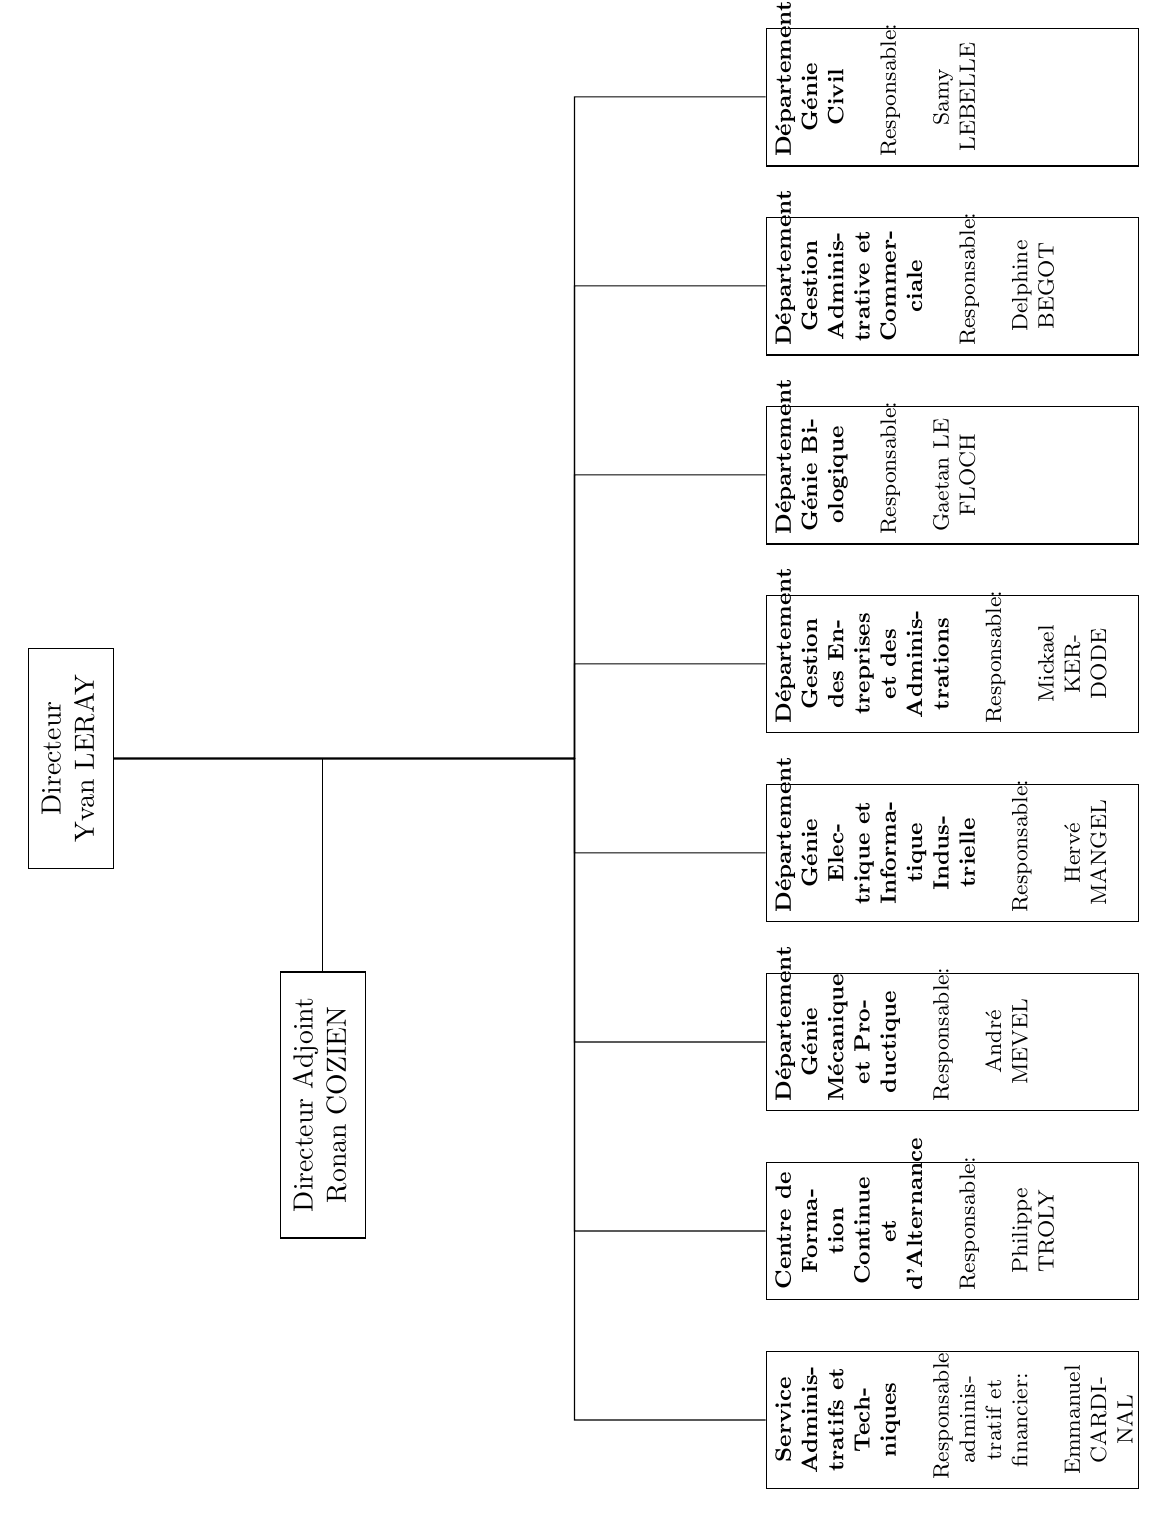
\begin{tikzpicture}[rotate=90]
\begin{scope}[xscale=1.6,yscale=1.6]
% description et nommage des noeuds
\node (AA) at (3.75,6) [rectangle,draw,rotate=90] {\begin{tabular}{c}Directeur\\Yvan LERAY\end{tabular} };
\node (PAF) at (1,4) [rectangle,draw,rotate=90] {\begin{tabular}{c}Directeur Adjoint\\Ronan COZIEN\end{tabular}};
\node (AAC) at (-1.5,-1) [rectangle,draw,rotate=90] {\begin{minipage}[t][4.5cm]{0.125\linewidth}\footnotesize \centering \textbf{Service Administratifs et Techniques} \\~\\
Responsable administratif et financier:\\~\\
Emmanuel CARDINAL
\end{minipage} };
\node (AAH) at (0,-1) [rectangle,draw,rotate=90] {\begin{minipage}[t][4.5cm]{0.125\linewidth}\footnotesize \centering \textbf{Centre de Formation Continue et d'Alternance} \\~\\
Responsable:\\~\\
Philippe TROLY
\end{minipage} };
\node (AAI) at (1.5,-1) [rectangle,draw,rotate=90] {\begin{minipage}[t][4.5cm]{0.125\linewidth}\footnotesize \centering \textbf{Département Génie Mécanique et Productique} \\~\\
Responsable:\\~\\
André MEVEL
\end{minipage} };
\node (AAJ) at (3,-1) [rectangle,draw,rotate=90] {\begin{minipage}[t][4.5cm]{0.125\linewidth}\footnotesize \centering \textbf{Département Génie Electrique et Informatique Industrielle} \\~\\
Responsable:\\~\\
Hervé MANGEL
\end{minipage} };

\node (AAK) at (4.5,-1) [rectangle,draw,rotate=90] {\begin{minipage}[t][4.5cm]{0.125\linewidth}\footnotesize \centering \textbf{Département Gestion des Entreprises et des Administrations} \\~\\
Responsable:\\~\\
Mickael KERDODE
\end{minipage} };

\node (AAL) at (6,-1) [rectangle,draw,rotate=90] {\begin{minipage}[t][4.5cm]{0.125\linewidth}\footnotesize \centering \textbf{Département Génie Biologique} \\~\\
Responsable:\\~\\
Gaetan LE FLOCH
\end{minipage} };

\node (AAM) at (7.5,-1) [rectangle,draw,rotate=90] {\begin{minipage}[t][4.5cm]{0.125\linewidth}\footnotesize \centering \textbf{Département Gestion Administrative et Commerciale} \\~\\
Responsable:\\~\\
Delphine BEGOT
\end{minipage} };

\node (AAN) at (9,-1) [rectangle,draw,rotate=90] {\begin{minipage}[t][4.5cm]{0.125\linewidth}\footnotesize \centering \textbf{Département Génie Civil} \\~\\
Responsable:\\~\\
Samy LEBELLE
\end{minipage} };

% description des arêtes
% -- arête rectiligne entre les noeuds nommés

\draw (AA) |- (PAF);
% |- départ vertical arrivée horizontale

% -| départ horizontal (du noeud de coordonnée (0,1)) arrivée verticale
\draw (AA) --++ (0,-4) -| (AAC);
\draw (AA) --++ (0,-4) -| (AAH);
\draw (AA) --++ (0,-4) -| (AAI);
\draw (AA) --++ (0,-4) -| (AAJ);
\draw (AA) --++ (0,-4) -| (AAK);
\draw (AA) --++ (0,-4) -| (AAL);
\draw (AA) --++ (0,-4) -| (AAM);
\draw (AA) --++ (0,-4) -| (AAN);
\end{scope}
\end{tikzpicture}
\end{figure}
\newpage

\mysubsection{Le Département Génie Electrique et Informatique Industrielle (GEII)}
\vspace{3em}
\begin{center}
\textbf{CHEF DE DEPARTEMENT:} Hervé Mangel

\end{center}
\begin{figure}[!h]
\centering
%\includegraphics[width=0.6\linewidth]{./img/herve.JPG}
\end{figure}
\begin{multicols*}{2}
\raggedcolumns
\renewcommand{\labelitemi}{\footnotesize $\blacksquare$}
\begin{itemize}
\itemsep 0.4cm
\item \textbf{Responsables:}\\

\begin{itemize}
\item Directeurs Etudes 1ère année: Laurence FIFRE - Mihai TELESCU
\item Directeurs Etudes 2ème année: Edgar ESPINOSA - Olivier CORRIO
\item Directeur Etudes Apprentissage: Sylvaine THIBERGE
\item Responsable des stages: Edgar ESPINOSA
\item Poursuites d'études: Marc LE ROY
\item Responsable emploi: Gérard LE MARC
\item Responsable Licence Pro MEE: Bruno JACCOUD
\item Responsable Licence Pro SARII: Vincent CHOQUEUSE - Olivier CORRIO
\item Secretariat : Philippe LE BERRIGOT\\
\end{itemize}
\item \textbf{Contact Département GEII:} Les coordonnées du département Génie électrique et Informatique Industrielle sont:\\

\begin{itemize}
\item Département GEII - IUT de Brest
Rue de Kergoat
CS 93837
29238 Brest Cedex 03
Tél: 02 98 01 60 68 / Fax: 02 98 01 66 43
Courriel: iutgeii@univ-brest.fr, Internet: http://www.iut-brest.fr/
\end{itemize}


\item \textbf{Contacts Licence SARII:} Le responsable pédagogique de la licence Professionnelle SARII peuvent être contactés par mail à l'adresse: \\

\begin{itemize}
\item vincent.choqueuse@univ-brest.fr.
\end{itemize}
\end{itemize}
\end{multicols*}


\begin{multicols}{2}
\noindent
\begin{itemize}
\item \textbf{Plan du département GEII}
\end{itemize}
\end{multicols}
\begin{figure}[!h]
%\includegraphics[width=1\linewidth]{./img/plan.jpg}
\end{figure}

\newpage

\renewcommand{\labelitemi}{-}
\mysection{L'ORGANISATION DES ETUDES}
\vspace{-0.5cm}
\begin{multicols*}{2}
\raggedcolumns
\mysubsection{Assiduité}

L'objectif de la formation réside dans une insertion professionnelle la plus rapide possible à l'issue de la Licence Professionnelle. Cet objectif ne pourra pas être atteint en cas d'absences multiples et répétées de la part de l'étudiant. Il est rappelé ci-après les seules situations qui ouvrent droit à une absence justifiée (ainsi que la nature des justificatifs réglementaires à fournir) :
\begin{itemize}
\item problèmes de santé liés à maladie ou accidents : certificat médical valant arrêt de travail pour maladie ou accident, bulletin d'hospitalisation ou pièces équivalentes.
\item examens ou concours avec justification par une convocation avec date et lieu de ces épreuves.
\item décès ou obsèques d'un proche (parents, ascendants, descendants, frères et soeurs) : photocopie du certificat de décès.
\item compétitions sportives (étudiant avec statut de sportif de haut niveau selon liste arrêtée par Ministère de l'Éducation Nationale) : photocopie des convocations avec date et lieu de ces compétitions.
\end{itemize}

Pour les étudiants de statut formation continue (Contrat de Professionnalisation ou autre), une copie de l'arrêt de travail sera à adresser au secrétariat du département GEII ou au responsable de la licence professionnelle SARII.

\mysubsection{Utilisation du téléphone portable}
Tout objet potentiellement bruyant tel que téléphone portable, montre..., doit être mis en veille pendant les enseignements, sous peine d'exclusion. Tout instrument électronique, téléphone portable, calculette... pouvant  stocker des fichiers ou donnant accès à internet sont formellement interdits pendant les examens. Tout enregistrement sonore ou visuel pendant les cours et examens est interdit.

\mysubsection{Fraude ou tentative de fraude lors d'un contrôle}

\textit{Circulaire n$^{o}$ 2000-033 - 1er alinéa ; article 22 ; Décret n$^{o}$ 92-657 modifié du 13/07/1992 .}\\

« En cas de flagrant délit de fraude ou tentative de fraude aux examens ou concours, le responsable de la salle prend toutes mesures pour faire cesser la fraude ou tentative de fraude sans interrompre la participation à l'épreuve du ou des candidats. Il saisit les pièces ou matériels permettant d'établir ultérieurement la réalité des faits. Il dresse un procès-verbal contresigné par les autres surveillants et par le ou les auteurs de la fraude ou de la tentative de fraude. En cas de refus de contresigner, mention est portée au procès-verbal.\\

\mysubsection{Charte anti plagiat de l'Université de Bretagne Occidentale (UBO)}

\textit{Approuvée par le Conseil d'administration de l'Université de Bretagne
Occidentale en date du 26 avril 2012 sur proposition du CEVU en date
du 13 mars 2012.}\\

\paragraph{Préambule: } L'Université de Bretagne Occidentale est engagée contre le plagiat, afin de garantir la qualité de ses diplômes et l'originalité des publications pédagogiques et scientifiques de ses personnels enseignants et/ou chercheurs. Les travaux, quels qu'ils soient (devoirs, compte-rendu, mémoire, cours, articles, thèses), réalisés aussi bien par les étudiants que par les personnels universitaires, doivent toujours avoir pour ambition de produire un savoir inédit et d'offrir une lecture nouvelle et personnelle d'un sujet. La présente charte définit les règles à respecter en la matière, par l'ensemble des étudiants et universitaires.

\paragraph{Article 1: } Les étudiants et les personnels sont informés que le plagiat constitue une
violation grave de l'éthique universitaire. Le plagiat consiste à reproduire
un texte, une partie d'un texte, toute production littéraire ou graphique, ou
des idées originales d'un auteur, sans lui en reconnaître la paternité par des
guillemets appropriés et par une indication bibliographique convenable.

\paragraph{Article 2: } Les étudiants et les personnels s'engagent de façon implicite par leur
inscription ou leur installation à l'université à ne pas commettre de plagiat
dans leurs travaux, quels qu'ils soient : devoirs et compte-rendu remis par
les étudiants à un enseignant, mémoire, cours, articles de recherche, thèse.
Le fait de commettre un plagiat en vue d'obtenir indûment une note, un
diplôme ou un grade universitaire est une circonstance aggravante. Le fait
de commettre un plagiat dans un document destiné à être publié, mémoire
de master ou de thèse, article à paraître dans une revue, est aussi une
circonstance aggravante. La reproduction d'une oeuvre originale sans le
consentement de l'auteur est de plus qualifiée juridiquement de
contrefaçon (articles L. 335-2 et L. 335-3 du code de la propriété
intellectuelle).

\paragraph{Article 3: } Les étudiants et les personnels s'engagent à citer, en respectant les règles de l'art, les travaux qu'ils utilisent ou reproduisent partiellement. Les reproductions de courts extraits en vue d'illustration. ou à des fins pédagogiques sont en effet autorisées sans nécessité de demander le consentement de l'auteur. Néanmoins, la méthodologie d'un travail universitaire. quel qu'il soit, implique que les emprunts soient clairement identifiés (guillemets) et que le nom de l'auteur et la source de [extrait soient mentionnés. Les travaux universitaires ne consistent pas en la reproduction d'une ou de plusieurs sources, mais doivent toujours avoir pour ambition de produire un savoir inédit et d'offrir une lecture nouvelle et personnelle du sujet.

\paragraph{Article 4:} L'Université de Bretagne Occidentale se réserve le droit de rechercher systématiquement les tentatives de plagiat par l'utilisation d'un logiciel de détection de plagiat. Les étudiants et les personnels s'engagent à communiquer, sur simple demande de l'Université. une version numérique de leurs travaux, afin de permettre cette détection.

\paragraph{Article 5:} Les manquements à la présente charte sont passibles de sanctions disciplinaires prévues au Code de l'Education et s'échelonnent de l'avertissement à l'exclusion définitive de tout établissement public d'enseignement supérieur. En cas de suspicion de plagiat. la section disciplinaire compétente de l'UBO sera saisie.
En plus de la procédure disciplinaire, les auteurs de plagiat s'exposent à des poursuites pénales pour contrefaçon. Toute information complémentaire sur les textes législatifs et réglementaires en vigueur et les règles de l'art pour la citation, peut être consultée dans le dossier plagiat sur le site de l'Université de Bretagne Occidentale.
\end{multicols*}

\newpage


\mysubsection{Présentation de la formation}
\vspace{-0.5cm}

\begin{multicols}{2}
\raggedcolumns

Tout en cherchant à préserver un bon niveau scientifique et technique sur un spectre assez large, la licence professionnelle SARII propose une spécialisation et des orientations "métiers" plus spécialisées dans les Systèmes Industriels et les Systèmes Automatisés et à la mise en oeuvre des Réseaux Industriels. Cette formation de niveau II répond à un besoin identifié exigeant :\\
\begin{itemize}
\item Une technicité affirmée, la maîtrise du champ technologique, des compétences élargies, une capacité à suivre l'évolution technologique du champ de compétences au sens large, ce qui suppose l'acquisition des fondamentaux.
\item Des qualités individuelles d'autonomie, d'initiative, de responsabilité, de capacité et de rigueur dans la conduite de projet et dans la gestion, l'aptitude à s'intégrer dans une équipe, à encadrer des équipes opérationnelles.\\
\end{itemize}
Globalement, les objectifs de la formation sont:
\begin{itemize}
\item Être capable de concevoir, faire réaliser et mettre en oeuvre un projet d'automatisation d'un système industriel.
\item Maîtriser les outils CAO et programmation spécifiques.
\item Savoir paramétrer et utiliser un bus de communication de terrain.
\item Maîtriser l'architecture d'un réseau d'automates programmables industriels
\item Connaître les éléments de base d'administration systèmes et réseaux (clients Windows avec serveurs).
\item Savoir mettre en place une supervision.
\item Appréhender les dispositifs et réseaux appliqués à la gestion technique et énergétique de bâtiments.
\end{itemize}
Outre une bonne maîtrise dans le choix et la mise en oeuvre, matérielle et logicielle, de solutions d'automatismes industriels, des compétences nouvelles recherchées sont liées à l'évolution du domaine : applications programmées embarquées (serveurs WEB embarqués), supervision, maintenance à distance,  gestion technique de bâtiment, programmation orientée objet.

La formation est structurée en 5 unités d'enseignement (UE). Ces UEs sont présentées dans le tableau~\ref{table2}. A noter que pour les étudiants inscrits dans un cycle de formation continue, la préparation complémentaire du CQPM (Certificat de Qualification Paritaire de la Métallurgie) "Assistant de projet en systèmes industriels informatisés" (CQPM MQ 95 10 07/26 0133) sera proposée. Cette possibilité apparaît comme un levier supplémentaire de reconnaissance du parcours en Licence Professionnelle par les entreprises avec un positionnement direct au sein des conventions collectives.


\newpage

\paragraph{Description des UEs}


Une unité d'enseignement est composée de Modules. Le contenu de chaque UE est décrit dans la Table~\ref{table2}. Les unités UE6 et UE7 ont un fonctionnement particulier.
\begin{itemize}
\item L'UE7 est réalisée au sein de l'entreprise. Cette UE sera évaluée par i) une soutenance orale des activités menées en entreprise,
ii) un rapport d'activités (rapport de stage pour les étudiants en formation initiale), et iii) appréciation du tuteur entreprise des compétences métiers (appréciation du déroulement du stage par le tuteur entreprise pour les étudiants en formation initiale).
\end{itemize}

\end{multicols}

\begin{table}[!h]
\centering
%% !TEX encoding = UTF-8 Unicode
\begin{tabular}{|c|p{0.6\linewidth}|c|c|}
\hline
\multicolumn{4}{|c|}{\textbf{UE1: Enseignements d'harmonisation (60 H)}}\\ 
\hline
\textbf{ID}&\textbf{Module}&\textbf{ECTS}&\textbf{Durée}\\ 
\hline
M104&Automatisme industriel
&0&20 H\\ 
M105&Programmation
&0&20 H\\ 
M106&Electronique Numérique
&0&20 H\\ 
\hline
\multicolumn{4}{|c|}{\textbf{UE2: Formation scientifique et technique (120 H)}}\\ 
\hline
\textbf{ID}&\textbf{Module}&\textbf{ECTS}&\textbf{Durée}\\ 
\hline
M201&SGBD (Systémes de Gestion de Base de Données)
&3&30 H\\ 
M202&Programmation orientée objet
&3&30 H\\ 
M203&Réseaux Industriels et Supervision
&3&30 H\\ 
M204&Instrumentation et Capteurs
&3&30 H\\ 
\hline
\multicolumn{4}{|c|}{\textbf{UE3: Formation professionnelle (150 H)}}\\ 
\hline
\textbf{ID}&\textbf{Module}&\textbf{ECTS}&\textbf{Durée}\\ 
\hline
M301&Processeurs spécialisés
&3&30 H\\ 
M302&Appareillage et Schéma Technique
&3&30 H\\ 
M303&Serveurs WEB Embarqués
&3&30 H\\ 
M304&Dispositifs et Réseaux appliqués à la gestion technique et énergétique du bâtiment.
&3&30 H\\ 
M305&Administration réseau
&3&30 H\\ 
\hline
\multicolumn{4}{|c|}{\textbf{UE4: Formation économique et sociale (120 H)}}\\ 
\hline
\textbf{ID}&\textbf{Module}&\textbf{ECTS}&\textbf{Durée}\\ 
\hline
M401&Conduite de projet/qualité
&2&20 H\\ 
M402&Economie et gestion
&2&20 H\\ 
M403&Connaissance de l'entreprise
&2&20 H\\ 
M404&Communication et insertion dans le milieu professionnel.
&3&30 H\\ 
M405&Anglais Professionnel et Technique
&3&30 H\\ 
\hline
\multicolumn{4}{|c|}{\textbf{UE5: Applications industrielles (150 H)}}\\ 
\hline
\textbf{ID}&\textbf{Module}&\textbf{ECTS}&\textbf{Durée}\\ 
\hline
M501&Projets tutorés
&6&150 H\\ 
M502&Stage Industriel
&15&560 H\\ 
\hline \end{tabular}
\caption{Description des Unités d'enseignement. Pour les étudiants/stagiaires, dans le cadre d'un contrat de professionnalisation, l'UE5 est réalisée en entreprise.}
\label{table2}
\end{table}


\newpage


%% Module à changer


    \input{./modules/{{module.code_scodoc}} }


\clearpage
\begin{multicols*}{2}
\raggedcolumns
\mysubsection{Contrôle des Connaissances}

Les modalités de contrôle des connaissances sont, conformément à la loi, arrêtées et portées à la connaissance des étudiants au plus tard à la fin du premier mois de l'année d'enseignement. Elles ne peuvent être modifiées en cours d'année. Les modalités du diplôme sont portées à la connaissance des étudiants dans ce document. Chaque étudiant se verra remettre ce document.\\


\paragraph{Modalités internes à une unité d'enseignement :}
Dans chaque unité d'enseignement, les aptitudes et l'acquisition des connaissances sont appréciées par un contrôle continu et régulier. Au sein de chaque unité d'enseignement, la compensation entre les notes obtenues aux différents modules s'effectue sans note éliminatoire.

\paragraph{Rattrapage :}
Si l'étudiant n'a pu satisfaire, pour une raison reconnue valable par le responsable de formation, à l'évaluation d'un ou plusieurs modules, il est autorisé à se représenter à une évaluation complémentaire de rattrapage.

\mysubsection{Stages pour la Formation Initiale}

Les stages effectués en lien avec le cursus de l'étudiant, et prévus dans l'habilitation, doivent faire l'objet d'une convention de stage obligatoire. Ces conventions doivent être signées par l'entreprise d'accueil, par l'étudiant, puis  (par ordre du Président de l'UBO) par le chef de département GEII (département Génie Électrique et Informatique Industrielle de l'IUT de Brest).

Ce stage est obligatoire car il fait partie de l'unité d'enseignement UE5. Les étudiants ayant le statut de salarié dans le cadre d'un contrat de professionnalisation (alternance) effectuent cette UE5 dans leur entreprise. Un rapport d'activités leur sera demandé et évalué pour valider cette unité d'enseignement.


\mysubsection{Évaluation de la Formation}

\paragraph{Évaluation des enseignements.}
Les modalités d'évaluation permettront au responsable de la formation de prendre connaissance de l'appréciation des étudiants par une évaluation des éléments pédagogiques mis en oeuvre et d'apprécier l'organisation des études. Une fiche d'appréciation est distribuée à chaque étudiant à la fin de chacun des modules et à la fin de la formation.

\paragraph{Évaluation de l'insertion professionnelle des étudiants.}
Une enquête menée 1 an après l'obtention du diplôme permettra de vérifier les caractéristiques et les évolutions de l'insertion et de faire évoluer la nature des grands domaines structurant les enseignements et les compétences attendues.
Ces enquêtes utiliseront les outils d

\newpage

\mysubsection{Modalités de contrôle des Connaissances: Année 2016-2017}

\paragraph{Jury}

Conformément à l'article 10 de l'arrêté du 17 novembre 1999:\\

La licence professionnelle est décernée aux étudiants qui ont obtenu à la fois une moyenne générale égale ou supérieure à 10 sur 20 à l'ensemble des unités d'enseignement.

La compensation entre éléments constitutifs d'une unité d'enseignement, d'une part, et les unités d'enseignement, d'autre part, s'effectue sans note éliminatoire.

Lorsqu'il n'a pas été satisfait au contrôle des connaissances et des aptitudes, l'étudiant peut conserver, à sa demande, le bénéfice des unités d'enseignement pour lesquelles il a obtenu une note égale ou supérieure à 8 sur 20.

La licence est décernée aux étudiants qui ont obtenu à la fois une moyenne générale égale ou supérieure à 10 à l'ensemble des unités d'enseignement, et une moyenne au moins égale à 10 à l'UE 5.

Lorsque la licence professionnelle n'a pas été obtenue, les unités d'enseignement dans lesquelles la moyenne de 10 a été obtenue sont capitalisables. Ces unités d'enseignement font l'objet d'une attestation délivrée par l'établissement.

La licence est délivrée sur proposition d'un jury désigné en application de l'article 17 de la loi du 26 janvier 1984. Ce jury comprend, pour au moins un quart et au plus la moitié, des professionnels des secteurs concernés par la licence professionnelle.

\paragraph{Conditions spécifiques UE1 et UE5 / LP SARI}

L'unité d'enseignement UE1 (coefficient 6) est constituée uniquement de modules d'harmonisation.

Si la moyenne de l'UE1 est inférieure à 10/20, aucun bonus n'est accordé. Si la moyenne de l'UE1 est supérieure ou égale à 10/20, un bonus vient s'ajouter à la moyenne générale. Ce bonus est calculé comme suit : Bonus = (moy UE1 - 10) / 10. Ainsi, l'étudiant peut bénéficier d'un bonus allant jusqu'à +1 point sur sa moyenne générale pour une moyenne de 20 / 20 dans l'UE1.
La moyenne de l'UE5 sera calculée à partir des modules M501(Projet tutoré) et M502 (Stage Industriel) selon les modalités suivantes :

\begin{itemize}
\item Pour les LP en FI : la note de M501 est celle du projet tuteuré de 150h.
\item Pour les LP en FC : la note de M501 est la même que celle de M502.
\end{itemize}

La délivrance du diplôme et la validation des unités d'enseignements sont prononcées après délibération du jury.
Il peut être attribué une mention : la mention assez bien est obtenue à partir de 12/20 de moyenne générale, la mention bien à partir de 14/20, la mention très bien à partir de 16/20.
e suivi existant déjà dans les IUT et à l'UBO. Un enseignant s'occupe plus particulièrement de l'aide à la recherche d'emploi et diligente les enquêtes.

\end{multicols*}

\newpage

\mysubsection{Modalités de contrôle des Connaissance: Année 2016-2017}

\begin{figure}[h]
\centering
%\includegraphics[width=0.78\textwidth]{img/MCC_2015.png}
\end{figure}

\clearpage


\mysubsection{ENT: Espace Numérique de Travail}
\vspace{-0.5cm}
\begin{multicols*}{2}
\raggedcolumns
\paragraph{Qu'est-ce que c'est ?}~\\

L'ENT est un dispositif global, en quelque sorte un bureau virtuel, qui fournit à chaque usager de l'établissement depuis n'importe quel accès internet où qu'il se trouve et quand il veut, un point d'accès, à travers les réseaux, à l'ensemble des ressources et services numériques en ligne en rapport avec son activité.\\

Que vous soyez étudiant ou personnel de l'UBO, vous pouvez accéder, à partir de cette page, à votre Environnement Numérique de Travail personnel. Une fois authentifié, vous trouverez les informations et services qui relèvent de votre statut et/ou fonction.
Le déploiement de cet ENT est destiné avant tout à vous aider dans votre travail et simplifier les accès à vos informations.

\paragraph{A quoi ça sert ?}~\\

Ainsi, selon le profil (étudiant ou personnel), il est possible de :
\begin{itemize}
\item se réinscrire en ligne,
\item lire et envoyer des messages électroniques,
\item effectuer des recherches documentaires,
\item accéder à son dossier personnel, ses fichiers (espace de stockage),
\item accéder à des ressources pédagogiques,
\item connaître les événements associatifs, culturels, sportifs,
\item accéder à des formulaires administratifs...
\end{itemize}

\paragraph{Comment y accéder ?}~\\


L'accès à l'ENT (et à d'autres services comme le C2i) nécessite le code personnel de votre passeport informatique.
Ce code est inscrit sur la carte étudiant qui vous est fournie en début d'année.
\noindent
\begin{center}
\fbox{\parbox{0.95\linewidth}{\textbf{ATTENTION :
Ne perdez surtout pas ce code Passeport informatique (notez-le en plusieurs endroits).
Il ne vous sera pas communiqué par la suite.}}}
\end{center}
\begin{enumerate}
\item Connectez-vous sur http://ent.univbrest.fr
\item Allez sur la rubrique [Passeport informatique] et laissez-vous guider
\item A la fin de la procédure, notez bien votre identifiant et votre mot de passe : ils vous serviront pour vous connecter à l'ENT, activer le Wifi, travailler sur le C2i, etc.
\end{enumerate}
En cas de perte du mot de passe, réactivez votre compte à partir de votre Passeport Informatique.
\paragraph{Les services proposés}~\\
\begin{enumerate}
\item Mon compte: pour changer votre mot de passe, consulter les adresses mail,...
\item Messagerie électronique
\item Dossier étudiant: vos coordonnées, formations suivies, notes,...
\item Ressources documentaires: Informations en relation avec la Bibliothèque Universitaire.
\item Espace de stockage personnel.
\item Espaces de stockage partagés
\item Actualités
\item Liste de diffusion
\end{enumerate}
L'ENT est en constante évolution.

\paragraph{Accès aux emplois du temps}~\\

Les emplois du temps sont accessibles à l'adresse: \url{https://iut.univ-brest.fr/hp/invite}

Lorsque vous accédez aux emplois du temps de l'extérieur, l'application web vous demandera de rentrer vos identifiants UBO. Une fois identifié, il suffit de sélectionner votre formation (Licence GEII3 ->SARII).

\end{multicols*}




\mysubsection{Charte Informatique}
\vspace{-0.5cm}
\begin{multicols*}{2}
\raggedcolumns
\textit{Charte du bon usage des réseaux et des systèmes informatiques de l'Université de Bretagne Occidentale (adoptée par le Conseil d'Administation de l'UBO du 30 mars 1995).}

\paragraph{Article 1- Domaines d'application :}
Les règles de bonne conduite de la présente charte s'appliquent à toute personne autorisée à utiliser les réseaux et les systèmes informatiques de l'UBO ainsi que les systèmes informatiques d'organismes extérieurs accessibles depuis l'UBO. Le Directeur du CRI-UBO et les responsables ayant en charge les systèmes informatiques au niveau des services peuvent édicter des règles de fonctionnement interne à leur service en cohérence avec la présente charte.
\paragraph{Article 2 - Conditions d'accès aux systèmes informatiques :}
Le droit d'accès à un système informatique est personnel et incessible. L'utilisation des moyens informatiques de l'UBO est limité à des activités de recherche, d'enseignement et de gestion.
\paragraph{Article 3 - Respect du caractère confidentiel des informations :}
Les utilisateurs ne doivent pas tenter de lire ou de copier les fichiers d'un autre utilisateur sans son autorisation (verbale ou écrite). Ils doivent également s'abstenir de toute tentative d'intercepter les communications privées entre utilisateurs, qu'elles se composent de courrier électronique ou de dialogue direct.
\paragraph{Article 4 - Respect des droits de propriété :}
Les utilisateurs doivent s'abstenir de faire des copies de tout logiciel autres que les logiciels gratuits du domaine public.
\paragraph{Article 5 - Respect des principes de fonctionnement des systèmes informatiques :}
Les utilisateurs ne doivent pas utiliser de comptes autres que ceux auxquels ils ont légitimement accès. Ils ne doivent pas non plus effectuer de manoeuvre qui aurait pour but de méprendre les autres utilisateurs sur leur identité. Ils doivent s'abstenir de toute tentative de s'approprier ou de déchiffrer le mot de passe d'un autre utilisateur, de modifier ou de détruire les fichiers d'un autre utilisateur et de limiter ou d'interdire l'accès aux systèmes informatiques d'un utilisateur autorisé. La conception d'un programme ayant de telles propriétés est également interdite.
\paragraph{Article 6 - Utilisation des réseaux informatiques :} Tout utilisateur d'un réseau informatique de l'UBO s'engage à ne pas effectuer d'opérations qui pourraient avoir pour conséquence :
\begin{itemize}
\item d'interrompre le fonctionnement normal du réseau ou d'un des systèmes connectés au réseau ;
\item de s'allouer des adresses IP sans autorisation ;
\item d'accéder à des informations privées concernant d'autres utilisateurs du réseau ;
\item de modifier ou de détruire des informations sur un des systèmes connectés au réseau ;
La conception d'un programme ayant de telles propriétés est également interdite.
\end{itemize}

Tout utilisateur désirant accéder à un réseau informatique de l'UBO via le réseau commuté doit en faire la demande écrite au Directeur du CRI-UBO. L'utilisateur s'engage à respecter les procédures de contrôle mise en place par le CRI-UBO.

\paragraph{Article 7 - Accès aux salles contenant le matériel informatique :}
Les utilisateurs s'engagent à respecter les règles d'accès aux salles contenant le matériel informatique.

\paragraph{Article 8 - Respect mutuel des individus entre eux :}
Les utilisateurs ne doivent pas persécuter un individu à l'aide d'outils électroniques.

\paragraph{Article 9 - Sanctions :}
Tout utilisateur n'ayant pas respecté les règles de bonne conduite énoncées dans la présente charte s'expose à des sanctions internes à l'UBO ou à des poursuites pénales (articles 462-2 à 462-9 du code pénal) suivant le cas.

\end{multicols*}

\renewcommand{\labelitemi}{-}
\mysection{LA VIE ETUDIANTE}
\vspace{-0.5cm}
\begin{multicols*}{2}
\raggedcolumns
\mysubsection{Restaurants universitaires}

Deux formules, resto U ou cafétéria, vous sont proposées.
\begin{itemize}
\item Resto U Brest Centre : 7 avenue Foch. Tél. 02 98 01 69 15
\item Resto U Kergoat : Rue du Commandant Vibert. Tél. 02 98 03 22 56
\item Resto U Le Bouguen : 2 bis avenue Le Gorgeu. Tél. 02 98 03 39 21
\end{itemize}
Ces restaurants sont ouverts du lundi au vendredi. Seul le RU de Kergoat reste ouvert le vendredi soir.\\
\begin{itemize}
\item Cafétéria de l'IUT : rue de Kergoat.
\item Cafétéria de Médecine : 22 avenue Camille Desmoulins
\item Cafétéria d'AES : 20 avenue Le Gorgeu
\item Cafétéria de l'UFR Sciences : 6 avenue Le Gorgeu\\
\end{itemize}
Ces cafétérias sont ouvertes en journée.

\mysubsection{Activités sportives}
L'Université vous propose plus de 40 activités sportives dans les domaines suivants :
\begin{itemize}
\item Sport de combat
\item Danses et expression
\item Remise en forme
\item Activités gymniques
\item Activités maîtrise de soi
\item Activités aquatiques
\item Raquettes
\item Sports collectifs
\end{itemize}
Pour plus amples renseignements, contacter le Service universitaire des activités physiques, sportives et de plein air (SUAPS). Tél.02 98 01 64 16 ou suaps@univ-brest.fr


\mysubsection{Médecine préventive}
Le Service Universitaire de Médecine Préventive et de Promotion de la Santé (SUMPPS) est situé au 13 rue de Lanrédec (Brest). Tél. 02 98 01 82 88.

\mysubsection{Bus tramway}
Pour une information, des horaires, les relais B, un itinéraire...: www.bibus.fr/

\end{multicols*}

\newpage
\mysection{PLANNING FORMATION CONTINUE}

\begin{figure}[h]
\centering
%\includegraphics[width=0.78\textwidth]{img/LP_SARII_planning.pdf}
\end{figure}



\end{document}

